\section{Implementation}

\subsection{Project Structure}

The simulation is implemented in C++. Implementation details will only be covered briefly here; the interested reader can visit \url{github.com/mattdutson/cherenkov_simulator} to view the source code. Any parameter values, where not explicitly given here, can be found in \texttt{Utility.h} or \texttt{Config.xml}. The project relies on three external libraries. CERN's ROOT libraries (\url{root.cern.ch}) are used for vector operations, coordinate transformations, fitting, and eigenvector finding among other things. The Boost libraries (\url{boost.org}) expand the core functionality of the C++ standard library. We only use the \texttt{property\_tree} class, which parses XML files into a hierarchical structure. Google Test (\url{github.com/google/googletest}) is used both to perform unit testing and to conveniently simulate individual shower cases. ROOT comes with a set of dynamic libraries which need to be referenced via environment variable during execution. Boost is header-only, and Google Test is built as a subdirectory of the project.

The top-level project directory, \texttt{cherenkov\_simulator}, contains the main executable, the XML configuration file, and subdirectories \texttt{cherenkov\_test} and \texttt{cherenkov\_lib}. \texttt{cherenkov\_test} contains unit tests and sample showers. Individual tests and showers can be run via command-line arguments to the \texttt{cherenkov\_test} executable (see the Google Test documentation). \texttt{cherenkov\_lib} implements all simulation, reconstruction, and Monte Carlo methods. It is compiled as a static library and linked to the other two executables.

\subsection{Configuration and Operation}

Simulation parameters are split between the executable and configuration file. Physical constants and most model parameters are hard coded in \texttt{Utility.h}. These values are unlikely to change from run to run. It's both cleaner and faster to hard code them than to re-parse on each execution. Other more variable parameters are stored in \texttt{Config.xml}. Among other things, they define the behavior of the simulation, the geometry of the detector, and noise removal thresholds. Running the main executable, \texttt{cherenkov\_simulator}, performs the Monte Carlo generation-simulation-reconstruction cycle. The first command-line argument is mandatory and specifies the path of the output file. If the user specified the output as \texttt{MonteCarlo}, then \texttt{MonteCarlo.root} and \texttt{MonteCarlo.csv} would be written to the current directory. The ROOT file contains plots of each shower, and the CSV summarizes the results of all reconstructions. The second argument is optional, and specifies a configuration file other than the default \texttt{Config.xml}. The third argument is also optional and sets the random number seed (an unsigned integer). This allows for repeatability between runs.

\subsection{Class Structure}
The following list summarizes the major classes defined in the implementation of \texttt{cherenkov\_lib}. \texttt{PhotonCount} is defined in \texttt{DataStructures.h}, and \texttt{Ray} and \texttt{Shower} are defined in \texttt{Geometric.h}. The remaining classes are defined in files which match their names.
\begin{itemize}
    \item \texttt{Ray}: A photon with a three-dimensional position and velocity. Keeps track of the current time, which is updated when the photon moves. Implements methods for reflection, refraction, and propagation.
    \item \texttt{Shower}: An extension of \texttt{Ray} which stores the primary particle's energy along with Gaisser-Hillas parameters. Implements methods for age, size, and atmospheric depth.
    \item \texttt{PhotonCount}: A three-dimensional array which is incremented in a certain (x, y, t) bin whenever a photon is detected. Stores linear and angular pixel size information, which is used when determining a pixel's direction with respect to the detector axis. A \texttt{PhotonCount::Iterator} can be used to move through the circular collection of valid pixels.
    \item \texttt{Simulator}: Simulates the development and detection of a shower. All member functions but the constructor are \texttt{const}. The constructor takes the parsed configuration file and stores required parameters as members.
    \item \texttt{Reconstructor}: Used for reconstructing a shower from the \texttt{PhotonCount} data produced by \texttt{Simulator}. Implements methods for the addition and subsequent filtering of noise. Similar to \texttt{Simulator} in structure.
    \item \texttt{MonteCarlo}: Used for performing the Monte Carlo cycle and generating random showers. Similar to \texttt{Simulator} in structure, but has a member \texttt{Simulator} and \texttt{Reconstructor}.
    \item \texttt{Analysis}: Defines a suite of static methods which can be used to plot and analyze the data in a \texttt{PhotonCount}.
    \item \texttt{Utility}: Implements miscellaneous static methods and defines hard-coded constants.
\end{itemize}
There are a handful of minor classes not listed here, most used as convenience wrappers for method parameters.

\section{Coordinate Systems and Surroundings} \label{sec:atmosphere}

The simulation uses three reference frames: the world frame, the detector frame, and the shower-detector frame. In all three, the telescope's center of curvature is the origin. This simplifies ray tracing and reduces transformations between frames to a rotation. In the world frame, the z-axis is perpendicular to the surface of the Earth. The y-axis is found by rotating the detector axis downward until it's horizontal, and the x-axis is given by the right hand rule. In the detector frame, the z-axis points along the detector axis, and the x-axis is shared with the world frame. The y-axis is again given by the right hand rule and typically points below the horizon. During reconstruction, a shower-detector plane is determined. The normal to this plane is the z-axis of the shower-detector frame. The x-axis must be in the world's x-y plane, and the y-axis is given by the right hand rule.

The ground is a simple plane with geometry defined in the configuration file. The user specifies, in the world frame, the plane's normal vector and a point which fixes its position. The normal vector doesn't necessarily align with the direction of atmospheric variation, which is $(0, 0, 1)$. The atmosphere is approximated with an exponential model. To derive this, we start with the ideal gas equation and a differential equation for pressure variation.
\begin{align}
    P &= \frac {\rho RT}{M} \\
    \text{d}P &= -\rho g \text{d}h
\end{align}
$M$ is the gas's molar mass, and $R$ is the ideal gas constant. If the temperature of the atmosphere is assumed constant, then the ideal gas equation gives a direct proportionality between $\rho$ and $P$, leading to the following solution:
\begin{equation}
\begin{aligned}
    \rho &= \rho_0 e^{-gMh / RT} \\
         &= \rho_0 e^{-h / H}.
\end{aligned}
\end{equation}
$\rho_0$ is the density at sea level, and $h$ is the elevation. $H$ is the ``scale height.'' Although it could be calculated directly by finding the atmosphere's molar mass and fixing a constant temperature, we chose to calculate it based on the atmospheric pressure at sea level.

\section{Random Shower Generation} \label{sec:shower_gen}

As discussed in Section \ref{sec:sim_summary}, each iteration of the Monte Carlo simulation begins with the random generation of a shower. This involves choosing a random geometry, energy, and set of Gaisser-Hillas parameters. The shower is first given a zenith angle $\theta$, which is distributed as $\cos{\theta}$ between zero and $\pi/2$. The shower is also given an azimuthal angle $\phi$, uniformly distributed between zero and $2\pi$. Together, these two angles completely define the direction of the shower. Recall that the impact point is the shower's closest approach to the detector (not to be confused with the ground reflection point). The allowed impact points lie on a disk centered at the detector and perpendicular to the shower direction. Points on the disk can be specified with polar coordinates $\beta$ and $R_p$. $\beta$ is distributed uniformly between zero and $2\pi$, and $R_p$ is chosen from a linear distribution between $R_\text{min}$ and $R_\text{max}$. $R_\text{min}$ = \texttt{impact\_min} and $R_\text{max}$ = \texttt{impact\_max} are defined in the configuration file. From the impact point, the shower is traced back to a starting point at depth $X_s$ = \texttt{start\_tracking}. Because the exponential atmosphere extends to infinity, $X_s$ must be positive. The starting height is found by integrating the atmospheric density from infinity and accounting for the zenith angle of the shower.
\begin{equation}
    h_s = -H \ln{\left(\frac{X_s \cos{\theta}}{\rho_0 H}\right)}
\end{equation}
Once the height is known, the starting $x$ and $y$ can be extrapolated using the shower direction and impact point.

\begin{figure}[!ht]
    \centering
    \frame{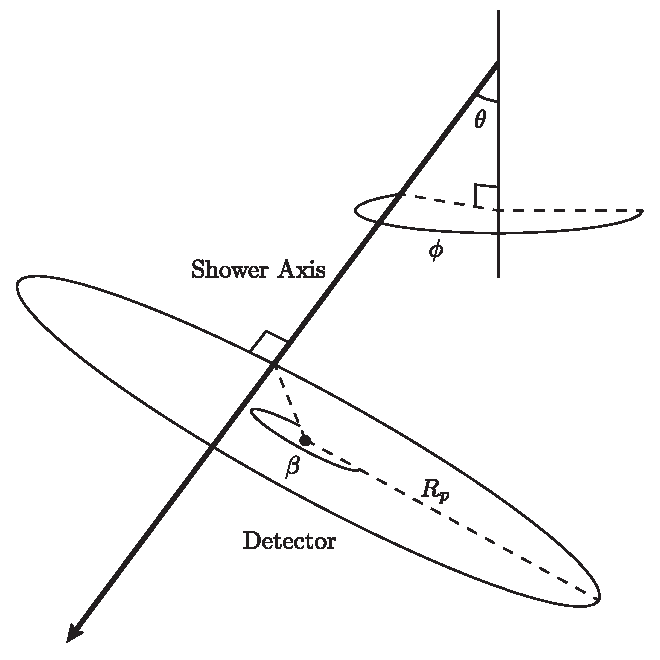
\includegraphics[width=0.8\textwidth]{ShowerGeneration}}
    \caption{Choosing the random geometry of a shower.}
\end{figure}

The primary energy is chosen from a power law, which has a slope, minimum, and maximum defined in the configuration file. The Gaisser-Hillas parameters (see Equation \ref{eq:gaisser_hillas}) can be calculated directly from the energy. $X_0$ is assigned a constant value of \SI{-70}{g/cm^2}. Although not physically realizable in an exponential atmosphere, this value gives a well-behaved Gaisser-Hillas function. The remaining parameters are calculated from the energy using
\begin{gather}
    X_\text{max} = 725 + 55.0 (\log_{10}(E) - 18.0) \\
    N_\text{max} = E / 1.3 \times 10^9.
\end{gather}
These expressions assume a proton primary and units of \si{eV} and \si{g/cm^2} \cite{abuzayyad2000hires}.

\section{Light Production} \label{sec:light_prod}

\subsection{Fluorescence Yield} \label{sec:fluorescence}

Once a shower has been initialized, it is stepped along its axis. At each step, the simulation determines the number of fluorescence and Cherenkov photons observed. Kakimoto gives the following parameterization of the number of fluorescence photons produced by a shower per unit per slant depth \cite{kakimoto1996yield}.
\begin{equation} \label{eq:fluorescence}
    Y_\text{fl} = \frac{\text{d}E / \text{d}X}{(\text{d}E / \text{d}X)_{\SI{1.4}{MeV}}}
        \left(\frac{A_1}{1 + \rho B_1 \sqrt{T}} + \frac{A_2}{1 + \rho B_2 \sqrt{T}}\right)
\end{equation}
The constants are given as $A_1 = \SI{890}{cm^2/g}$, $A_2 = \SI{550}{cm^2/g}$, $B_1 = \num{1.85e3}$ \si{cm^3/g.K^{1/2}}, and $B_2 = \SI{6.50e3}{cm^3/g.K^{1/2}}$. $\text{d}E / \text{d}X$ is the energy deposit, the rate per slant depth at which the shower loses energy to the atmosphere. $(\text{d}E / \text{d}X)_{\SI{1.4}{MeV}}$ is the energy deposit of a single \SI{1.4}{MeV} electron, given as \SI{1.6}{MeV.cm^2/g}. Kakimoto's original parameterization of $Y_\text{fl}$ came with a factor of $\rho$, and was expressed per unit distance. Dividing by $\rho$ gives the formula in units of slant depth instead.

Nerling gives a parameterization of the energy deposit as a function of shower age \cite{nerling2006electron}. Age is a unitless quantity defined as $s = 3X / (X + 2X_\text{max})$.
\begin{gather} \label{eq:deposit}
    \diff{E}{X}(X) = \alpha_\text{eff}(X, E > E_\text{cut}) \cdot N(X, E > E_\text{cut}) \\
    \alpha_\text{eff}(s) = \frac{c_1}{(c_2 + s)^{c_3}} + c_4 + c_5 \cdot s
\end{gather}
$\alpha_\text{eff}$ is the effective ionization loss rate, representing the energy deposit of a single particle. The constants are given as $c_1 = \num{3.90883}$, $c_2 = \num{1.05301}$, $c_3 = \num{9.91717}$, $c_4 = \num{2.41715}$, and $c_5 = \num{0.13180}$. These values give $\alpha_\text{eff}$ in units \si{MeV.cm^2/g}. Note that both terms in Equation \ref{eq:deposit} depend on $E_\text{cut}$, a simulation cutoff used by CORSIKA. The formula for $\alpha_\text{eff}$ assumes a cutoff of \SI{1}{MeV}. For reasons discussed in Section \ref{sec:cherenkov}, it is sufficient to use the cutoff-independent Gaisser-Hillas parameterization in place of $N(X, E > E_\text{cut})$. With this, the fluorescence yield obtains its final form.
\begin{equation} \label{eq:fluor}
    Y_\text{fl} = \frac{\alpha_\text{eff}(s) \cdot N(X)}{(\text{d}E / \text{d}X)_{\SI{1.4}{MeV}}} 
        \left(\frac{A_1}{1 + \rho B_1 \sqrt{T}} + \frac{A_2}{1 + \rho B_2 \sqrt{T}}\right)
\end{equation}

\subsection{Cherenkov Yield} \label{sec:cherenkov}

The Cherenkov yield for an individual shower electron varies with its energy. Nerling gives the following parameterization of the Cherenkov yield of a single electron \cite{nerling2006electron}:
\begin{equation}
    Y_\text{cv}(h, E) = \frac{2 \pi \alpha Z^2}{\rho(h)} 
        \int^{\lambda_2}_{\lambda_1} \left(1 - \frac{1}{n^2(h, \lambda) \beta^2}\right) 
        \frac{\text{d} \lambda}{\lambda^2}
\end{equation}
$\alpha$ is the fine structure constant, $Z = 1$, $n$ is the atmospheric index of refraction, and $\beta = v / c$. $(\lambda_1, \lambda_2)$ is the range of wavelengths to which the detector is sensitive, something like 300-400 \si{nm}. Because the dependence of $n$ on wavelength is small and $n \approx 1$, the yield can be simplified. We define $\delta(h) = 1 - n(h)$.
\begin{equation}
\begin{gathered}
    1 - (n \beta)^{-2} \approx 2 \delta - \frac{m^2 c^4}{E^2} \\
    Y_\text{cv}(h, E) \approx \frac{2 \pi \alpha Z^2}{\rho(h)} 
        \left(\delta(h) - \frac{m^2 c^4}{E^2}\right)
        \left(\frac{1}{\lambda_1} - \frac{1}{\lambda_2}\right)
\end{gathered}
\end{equation}
The Cherenkov yield for the entire shower is calculated by averaging the single particle yield over the electron energy spectrum, then multiplying that expectation value by the total number of electrons. This gives the total number of Cherenkov photons produced per slant depth.
\begin{equation} \label{eq:ckv_yield}
    \diff{N_\gamma}{X} = N(X) \int^{\infty}_{\ln{E_\text{thr}}} 
        Y_\text{cv}(h, E) f_e(s, E) \text{d} \ln{E}
\end{equation}
$E_\text{thr} = m_e c^2 / \sqrt{2 \delta}$ is the threshold below which an electron will not produce Cherenkov radiation. Nerling gives a parameterization of the electron energy spectrum as a function of shower age \cite{nerling2006electron}.
\begin{gather}
    f_e(s, E) = a_0 \cdot \frac{E}{(E + a_1)(E + a_2)^s} \\
    \begin{aligned}
        a_0 &= k_0 \exp(k_1 \cdot s + k_2 \cdot s^2) \\
        a_1 &= \num{6.42522} - \num{1.53183} \cdot s \\
        a_2 &= \num{168.168} - \num{42.1368} \cdot s
    \end{aligned}
\end{gather}
$E$ is assumed to have units of \si{MeV}. The choice of the normalization constant $a_0$ depends on the CORSIKA cutoff energy. It is chosen such that
\begin{equation}
    \int^{\infty}_{\ln{E_\text{cut}}} f_e(X, E) \text{d} \ln{E} = 1.
\end{equation}
As for the fluorescence yield, we assume $E_\text{cut} = \SI{1}{MeV}$. This cutoff gives  $k_0 = \num{0.145098}$, $k_1 = \num{6.20114}$ , and $k_2 = \num{-0.596851}$. Equation \ref{eq:ckv_yield} must be integrated numerically. To improve the speed and robustness of this integration, its upper limit is set to the natural log of the total shower energy. The spectrum remains well normalized under this approximation. 

There is a subtlety to be addressed regarding the CORSIKA cutoff energy. The normalization of the electron energy spectrum depends on the cutoff, which means that our Cherenkov yield differs depending on what we choose as the cutoff. We could correct for this by using $N_\text{ch}(E > E_\text{cut})$ instead of the Gaisser-Hillas number. Figure \ref{fig:corsika_cut} demonstrates the dependence of $N_\text{max}$ on the cutoff energy, where a cutoff of zero corresponds to the unmodified Gaisser-Hillas parameterization \cite{nerling2006electron}. Due to the small fractional change from zero to $E_\text{cut} = \SI{1}{MeV}$, the Gaisser-Hillas value is used without correction.

\begin{figure}[!ht]
    \label{fig:corsika_cut}
    \centering
    \includegraphics[width=0.8\textwidth]{CorsikaCutoff}
    \caption{The dependence of $N_\text{ch}(E > E_\text{cut})$ on $E_\text{cut}$, taken from Nerling \cite{nerling2006electron}. Note the relatively small fractional change from zero to \SI{1}{MeV}.}
\end{figure}

\section{Ray Tracing}

\subsection{Random Ray Generation} \label{sec:generation}

Once the number of observed photons is known, each must be ray-traced to the detector. Fluorescence photons are emitted isotropically and travel directly from the shower to the detector. The fraction captured is equal to the fraction of a sphere covered by the detector.
\begin{equation} \label{eq:fluor_frac}
    f_\text{fl} = \frac{r^2}{4d^2} \cos{\theta}
\end{equation}
$\theta$ is the angle between the detector axis and the emission point, $r$ the radius of the stop, and $d$ the distance from the detector to the emission point. This fraction is multiplied by the mirror reflectance, photomultiplier quantum efficiency, and wavelength filter transmittance to convert the number of photons to the number of detected photoelectrons. Physically, these inefficiencies occur within the detector, but it is equivalent to apply them before ray tracing. The user may define a thinning rate, $T = $ \texttt{fluor\_thin}, which reduces the number of unique simulated photons by a factor of $T$. Each of the $N / T$ photons is recorded $T$ times when it reaches the detector. The ray for each detected fluorescence photon is placed at the location of the shower, and randomly shifted up or down within the current step. The starting time of the ray is adjusted accordingly. Each ray is traced to a random point on the stop.

Unlike fluorescence, Cherenkov photons must be reflected from the ground. When determining the fraction seen, it is assumed that most are reflected near the ground impact of the shower core. The Lambertian model of diffuse reflection is used, which assumes that the amount of light captured scales like the apparent size of the surface. Defining $f_\text{cv}$ as the Cherenkov fraction, we write $f_\text{cv} = A \cos{\phi} \text{d} \Omega$, where $\phi$ is the angle of the observer with respect to the ground's normal vector. Integrating this over a half sphere gives the normalization factor $A = 1 / \pi$. Let $f_s$ be the fraction of a sphere covered by the detector relative to the ground reflectance point, with the same form as Equation \ref{eq:fluor_frac}. Assuming $f_s$ is small, we can write $\text{d}\Omega = 4 \pi f_s$. Therefore,
\begin{equation}
    f_\text{cv} = 4 \cos{\phi} f_s.
\end{equation}
The detector efficiency and computational thinning are applied as they were for fluorescence. The angle between Cherenkov photons and the shower axis obeys the following distribution given by Stratton \cite{stratton2012ta}:
\begin{equation} \label{eq:ckv_angle}
\begin{gathered}
    A(\theta) = e^{-\theta / \theta_c} \\
    \theta_c = 0.83 E_\text{thr}^{-0.67}.
\end{gathered}
\end{equation}
For each simulated Cherenkov photon, a direction is chosen from this distribution, and the position is found via the same shifting method used for fluorescence. These photons are propagated until they collide with the ground plane, where they are reflected to random locations on the stop.

\subsection{Detector Optics} \label{sec:optics}

After reaching the stop, both fluorescence and Cherenkov photons must be traced through the detector optics. This involves refraction by the Schmidt corrector. The shape of the corrector is given by Malacara \cite{malacara2004optics}.
\begin{equation}
    Z(S) = \frac{S^2}{4(n - 1)r_m^3}(S^2 - S_\text{max}^2)
\end{equation}
$S$ is the distance from the axis, $n$ the lens' index of refraction, $r_m$ mirror's radius of curvature, and $S_\text{max}$ the radius of the stop. As explained in Section \ref{sec:intro_recon}, the quadratic term and inner portion of the corrector are removed. A local minimum of $Z(S)$ occurs at $S_\text{max} / \sqrt{2}$, and is set as the inner boundary of the corrector.
\begin{equation}
Z(S)=
    \begin{cases}
    \frac{S^4}{4(n - 1)r_m^3} & \text{ if } S > S_\text{max} / \sqrt{2} \\
    0 & \text{ if } S \leq S_\text{max} / \sqrt{2}
    \end{cases}
\end{equation}
Performing the refraction requires finding lens normal $\vec{n}_l$ for any $(x, y)$ on the stop. If $S \leq S_\text{max} / \sqrt{2}$, the normal is $(0, 0, 1)$. If $S > S_\text{max} / \sqrt{2}$, then the x and y components must point back toward the z-axis, so they are set to $-x$ and $-y$. The ratio of the z component to the planar component is $1 / Z'(S)$, which is guaranteed to be non-infinite for $S > S_\text{max} / \sqrt{2}$. Therefore, the normal vector is
\begin{equation}
\begin{aligned}
\vec{n}_l &= \left(\frac{S}{Z'(S)}, -x, -y\right) \\
          &= \left(\frac{(n - 1)r_m^3}{S^2}, -x, -y\right).
\end{aligned}
\end{equation}
This can be normalized to obtain $\hat{n}_l$, the unit normal vector. If the incident ray is not parallel to $\hat{n}_l$ and has direction $\vec{d}$, then the axis of rotation for the refraction is $\hat{n}_l \times \vec{d}$. The angle of rotation about this axis is determined by Snell's law. When refracting across the flat back surface of the corrector, the same procedure is used, but with a normal vector of $(0, 0, -1)$ and a check for total internal reflection. The two refractions are performed back-to-back, without accounting for the finite corrector thickness.

Rays are then traced to their intersection with the spherical mirror. The sphere is centered at the origin and defined by $x^2 + y^2 + z^2 = r_m^2$. Given the ray's starting position $(x_0, y_0, z_0)$ and velocity $(v_x, v_y, v_z)$, the times when the ray will cross the sphere can be found by solving
\begin{equation}
    (x_0 + v_x t)^2 + (y_0 + v_y t)^2 + (z_0 + v_z t)^2 = r_m^2.
\end{equation}
If there are two roots, then the one giving a more negative z-value is chosen. If there are no roots or the intersection points lie outside the edge of the mirror (which is only a section of the sphere), the ray is thrown out. Valid rays are traced to their reflection points, checking for collision with the back of the focal surface. Reflection subtracts $2 \vec{v} \cdot \hat{n}_m$ from the velocity, where $\hat{n}_m$ is the mirror normal at the reflection point. Because the center of curvature is the origin, $\hat{n}_m$ is simply the negative unit position of the reflection point.

Rays are traced to the spherical detection surface with the same method used for the mirror. Any photons outside the boundaries of the pixel array are thrown out. If the position of the focal impact point is $\vec{f}$, then the pixel bins $b_x$ and $b_y$ can be found using the following:
\begin{gather}
    \begin{gathered}
        \theta = \arctan{\frac{f_y}{f_z}} \\
        \phi = \arctan{\frac{f_x}{f_z}}
    \end{gathered} \qquad
    \begin{gathered}
        b_y = \left\lfloor \frac{\theta}{\Delta \alpha} \right\rfloor + n \\
        b_x = \left\lfloor \frac{\phi}{\alpha \cos{\theta}} \right\rfloor + n
    \end{gathered}
\end{gather}
$2n$ is the diameter of the array in pixels, and $\Delta \alpha$ is the angular size of each pixel. $b_t$ is determined with a straightforward temporal binning. Certain reasonable limits are placed on the minimum and maximum allowed times so the underlying data structure can be given a finite size. If the time is within these bounds, the counter at the $(b_x, b_y, b_t)$ bin is incremented by the thinning level.

\section{Addition and Filtering of Noise} \label{sec:noise}

Night sky background noise obeys a Poisson distribution.
\begin{equation} \label{eq:poisson}
    P(k: \lambda) = e^{-\lambda}\frac{\lambda^k}{k!}
\end{equation}
$\lambda$ is the mean rate and $k$ is a particular number of noise photons. Noise is added by iterating through each $(b_x, b_y, b_t)$ bin and randomly sampling from the Poisson distribution, where
\begin{equation}
    \lambda = \Omega_p  A_s  T_b  \mu.
\end{equation}
$A_s$ is the area of the stop, $T_b$ the time per bin, and $\Omega_p$ the solid angle of a single pixel. $\mu = \SI{4.9e5}{sr^{-1}.cm^{-2}.s^{-1}}$ is the night sky noise level. This value is based on Telescope Array observations of 6 photoelectrons per \SI{100}{ns} per square degree per \SI{4}{m^2}. Noise from pixels pointing toward the ground also obeys a Poisson distribution, but the mean is lowered by a factor of ten. Most noise filtration steps involve comparing signal values to thresholds, which are computed as multiples of $\sigma$. For a Poisson distribution, $\sigma=\sqrt{\lambda}$. However, a direct application of this formula tends to give more lenient thresholds than would be found with the same multiple of $\sigma$ on a Gaussian. To solve this problem, an upper bound is chosen for the Poisson threshold probability. For a $3\sigma$ threshold, the $3\sigma$ tail of a Gaussian is integrated to give probability \num{0.0014}. To match this, the Poisson threshold is increased until the above-threshold probability is less than \num{0.0014}.

Noise filtration begins with the uniform subtraction of $\lambda$ from each bin. Triggering logic is then applied to omit frames and showers where no significant signal is seen. In each time frame, the largest cluster of signals above $6\sigma$ is found. If this cluster contains more than five pixels, the frame is triggered. If no frames are triggered, then a reconstruction is not attempted. Otherwise, a set of anchor points is chosen, starting with any bins above $6\sigma$ which are in a triggered frame. A shower-detector plane is fit to the anchor points (see Section \ref{sec:recon}). Any anchor points more than some angle $\theta_\text{max}$ from the plane are removed, according to
\begin{equation}
    \arcsin(\hat{n}_p \cdot \hat{v_i}) > \theta_\text{max}.
\end{equation}
$\hat{n}_p$ is the plane normal vector, and $\hat{v_i}$ the pointing direction of a particular pixel. The remaining anchors are used as the starting points of a breadth-first traversal of the 3D histogram. The traversal bleeds outward from anchor points through any $3\sigma$ bins which occupy the eight spatially adjacent or two temporally adjacent spaces. All anchor points and accessible $3\sigma$ points are considered non-noise; everything else is removed.

\section{Reconstruction} \label{sec:recon}

If a pixel has direction $\hat{v_i}$, and the shower-detector plane has normal vector $\hat{n}_p$, then the deviation of that pixel from the plane can be measured by $(\hat{v_i} \cdot \hat{n}_p)^2$. This gives the following $\chi^2$ for the shower-detector plane, taken with modification from Stratton:
\begin{equation}
    \chi^2 = \sum_i  N_i \cdot (\hat{\nu_i} \cdot \hat{n})^2.
\end{equation}
$N_i$ is the total number of non-noise photoelectrons observed by the pixel \cite{stratton2012ta}. Stratton performs the summation only over ``good tubes.'' The choice of good tubes depends partially on the choice of the shower-detector plane, so the fit must be performed iteratively. Our good tubes have already been determined using the noise filtration methods from the previous section, eliminating the need for an iterative minimization. The minimum of the chi square can be found analytically by taking $\hat{n}_p$ to be the eigenvector of a symmetric matrix $M$ with the smallest eigenvalue, where
\begin{equation}
    M_{jk} = \sum_i  N_i \nu_{ij} \nu_{jk}.
\end{equation}

The monocular fit uses the analytic time profile of Equation \ref{eq:time_prof}. Each pixel's $\chi_i$ is found by rotating its direction to the shower-detector frame and taking the angle with the x-axis. $t_i$ is the mean of the photon arrival times. Due to the binned nature of the data, a Sheppard correction of $T_b^2 / 12$ is added to the variance of the mean. $R_p$, $\psi$, and $t_0$ can be found by fitting Equation \ref{eq:time_prof} against the $(\chi_i, t_i)$ points. Once this monocular fit has been performed, a decision is made whether to perform the Cherenkov fit. The monocular $R_p$ and $\psi$ can be used to estimate the ground impact point of the shower. If the impact point is visible by the detector and at least some angle $\theta_\text{min}$ from the edge of the field of view, a search is performed over all below-horizon pixels and the brightest pixel is found. If the brightest pixel has a signal above $6\sigma$, it is selected as the reflectance point and its direction is extended to the ground. The Cherenkov reconstruction is then performed similarly to the monocular reconstruction, with the only difference being the replacement of $R_p$ with $d \sin(\psi + \alpha)$ (see Equation \ref{eq:ckv_relation}).